\documentclass[journal=jacsat,manuscript=article]{achemso}

\usepackage[utf8]{inputenc}
\usepackage[version=3]{mhchem}
\usepackage{xcolor}
\usepackage{hyperref}
\usepackage{listings}

\let\epsilon=\varepsilon


\author{Romain Gaillac}
\affiliation[XXXXX]
{XXXXXX}
\author{Siwar Chibani}
\affiliation[PSL University]
{Chimie ParisTech, PSL University, CNRS, Institut de Recherche de Chimie Paris, 75005 Paris, France}
\author{Fran\c{c}ois-Xavier Coudert}
\email{fx.coudert@chimieparistech.psl.eu}
\affiliation[PSL University]
{Chimie ParisTech, PSL University, CNRS, Institut de Recherche de Chimie Paris, 75005 Paris, France}


\title{Prediction Auxeticity of Zeolite Frameworks by Machine Learning: Supporting Information}

\begin{document}

\begin{figure}[ht!]\centering
		\begin{lstlisting}
		quartz
		CRYSTAL
		0 0 0
		154
		4.95304267 5.45063836 120.0
		2
		14 0.468244242584 -5.551115e-17 -0.333333333333
		8 0.411357593826 0.270377816093 -0.217333686507
		ELASTCON
		MAXCYCLE
		1000
		PREOPTGEOM
		END
		BASISSET
		POB-TZVP
		DFT
		PBESOLXC
		ENDDFT
		FMIXING
		40
		LEVSHIFT
		5 0
		GRIMME
		0.75 20. 25.
		2
		14 9.23 1.716
		8 0.70 1.342
		SHRINK
		5 5
		END
		\end{lstlisting}
		%BIPOSIZE
		%40000000
		%EXCHSIZE
		%40000000
		\caption{\label{file_crystal} 
		Representative input file for calculations with the C\textsc{rystal}14 software package (here for quartz). Input data are given in the following order: geometrical information (space group number, cell parameters, fractional coordinates of non-equivalent atoms), keywords defining the calculation type (here computation of elastic properties, preceded by a geometry optimization), basis set information, exchange-correlation functional, technical parameters to facilitate convergence, and, here, inclusion of dispersion corrections), and finally shrink parameter, which depends on system size (set so that the minimum lattice parameter multiplied by it gives a value above 20).
		}
		\end{figure}
		
		
\begin{figure}[ht!]\centering
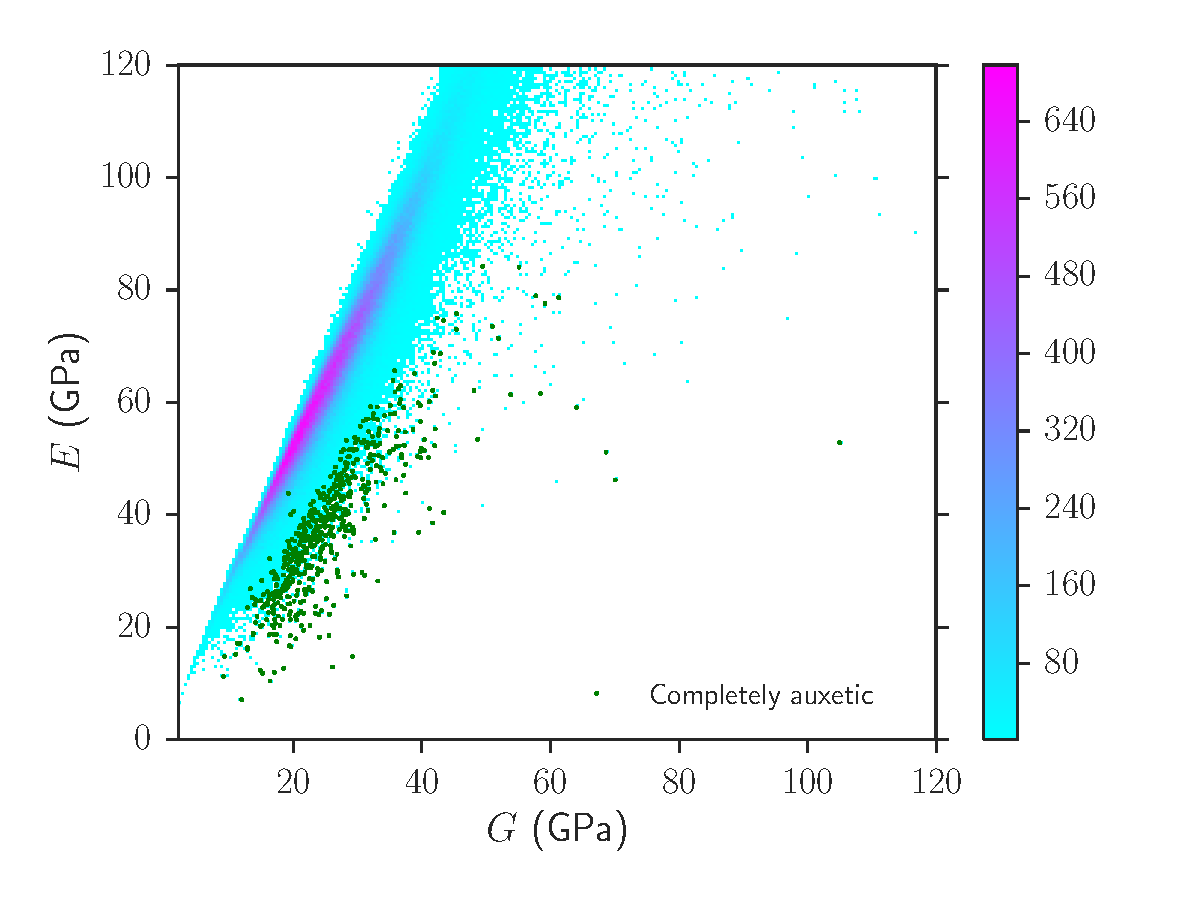
\includegraphics[clip,trim=0.7cm 0.7cm 1.3cm 0.7cm,width=0.495\textwidth]{zeolite_study_1_1}
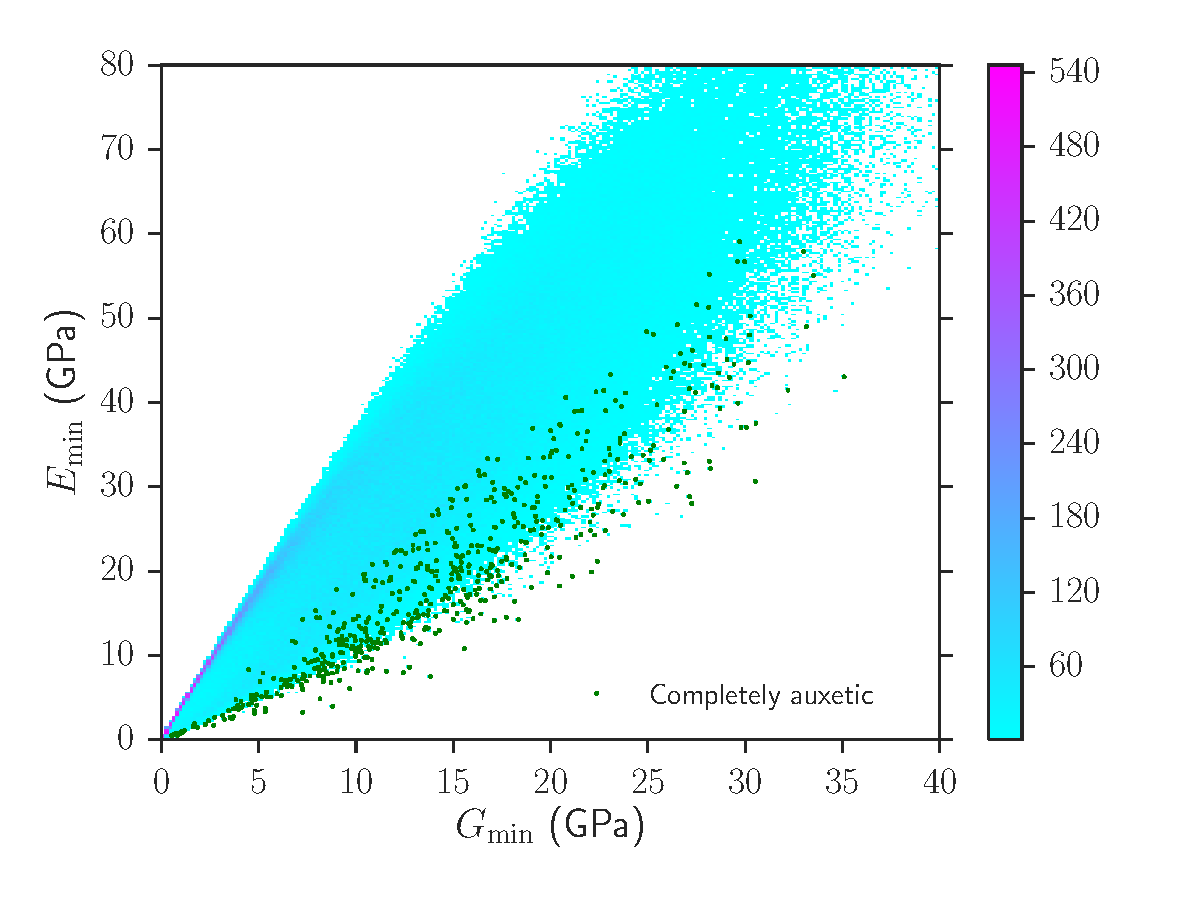
\includegraphics[clip,trim=0.5cm 0.7cm 1.5cm 0.7cm,width=0.495\textwidth]{zeolite_study_1_2}
\caption{Correlation heatmap between the average shear modulus $G$ (GPa) and the average Young's modulus $E$ (GPa) (left) and their minima (right).
\label{corr_G_E_totalaux}}
\end{figure}
		
\end{document}